%%%%%%%%%%%%%%%%%%%%%%%%%%%%%%%%%%%%%%%%%%%%%%%%%%%%%%%%%%%%%%%%
% %
% Due Date %
% Andrew Gibson %
% ECE 351 lab, Section 53 %
% Lab 2 %
% Due 31 Jan 2023 %
% User-Defined Functions %
%https://github.com/gibs0630/ECE351\_Code %
%https://github.com/gibs0630/ECE351\_Reports %
% %
%%%%%%%%%%%%%%%%%%%%%%%%%%%%%%%%%%%%%%%%%%%%%%%%%%%%%%%%%%%%%%%%

\documentclass[12pt,a4paper]{article}
\usepackage[utf8]{inputenc}
\usepackage[greek,english]{babel}
\usepackage{alphabeta} 
\usepackage[pdftex]{graphicx}
\usepackage[top=1in, bottom=1in, left=1in, right=1in]{geometry}
\linespread{1.06}
\setlength{\parskip}{8pt plus2pt minus2pt}
\widowpenalty 10000
\clubpenalty 10000
\newcommand{\eat}[1]{}
\newcommand{\HRule}{\rule{\linewidth}{0.5mm}}
\usepackage[official]{eurosym}
\usepackage{enumitem}
\setlist{nolistsep,noitemsep}
\usepackage[hidelinks]{hyperref}
\usepackage{cite}
\usepackage{lipsum}


\newcommand{\Q}{\bigskip\bfseries Q: }
\newcommand{\A}{\par\textbf{A:} \normalfont}

\hypersetup{colorlinks=true, linkcolor=black, urlcolor=blue}

\begin{document}
%===========================================================
\begin{titlepage}
\begin{center}
% Top 
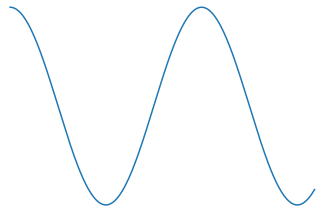
\includegraphics[width=0.55\textwidth]{titlepage_image.png}~\\[2cm]
% Title
\HRule \\[0.4cm]
{ \LARGE 
  \textbf{Project Report for ECE 351}\\[0.4cm]
  \emph{Lab 2: User-Defined Functions}\\[0.4cm]
}
\HRule \\[1.5cm]
% Author
{ \large
  Andrew Gibson \\[0.1cm]
  17 January 2023\\[0.1cm]
  \url{https://github.com/gibs0630/ECE351\_Code}\\[0.1cm]
  \url{https://github.com/gibs0630/ECE351\_Reports}\\[0.1cm]
  %#\texttt{user@cut.ac.cy}
}
\vfill
%\textsc{\Large Cyprus University of Technology}\\[0.4cm]\textsc{\large Department of Electrical Engineering,\\Computer Engineering \& Informatics}\\[0.4cm]
% Bottom
{\large }
 
\end{center}
\end{titlepage}
%\begin{abstract}
%\lipsum[1-2]
%\addtocontents{toc}{\protect\thispagestyle{empty}}
%\end{abstract}
\newpage
%===========================================================
\tableofcontents
\addtocontents{toc}{\protect\thispagestyle{empty}}
\newpage
\setcounter{page}{1}
%===========================================================
%===========================================================
\section{Introduction}\label{sec:intro}
On a computer, it may be easier to apply a function to discrete values then to a continuous function.  Continuous functions may not be handle-able on the computer hardware if it gets complex, or if it has to deal with noise. Python has a few libraries, notably numpy and matplotlib, that allows for the ease of managing and plotting data from large arrays.  The library numpy adds an array that has a simple to code piece-wise calculations, which can allow operations such as translating, scaling, and discrete differentiation.  The library matplotlib allows for simple to code plotting.

\section{Equations}\label{sec:lit-rev}
Formula's used
unit step function
\[
u(x) = \left\{
        \begin{array}{ll}
            0 & \quad t < 0 \\
            1 & \quad t \geq 0
        \end{array}
    \right.
\]
ramp function
\[
r(x) = \left\{
        \begin{array}{ll}
            0 & \quad t < 0 \\
            t & \quad t \geq 0
        \end{array}
    \right.
\]


functions from lab
\[func2(t) = r(t)-r(t-3)+5u(t-3)-2u(t-6)-2r(t-6)\]


\section{Methodology}\label{sec:meth}
This lab had us create plots Using python.  Graphs that were created were with a cosine wave, unit step, ramp, and a combination of step and ramp, along with some transforms of a combination of steps and ramps.

First an array of evenly spaced values for time, was created. Each of those discrete values of time were then plugged into a function of time to create a second array.

The arrays from the numpy library allow for ease of vertical translation by simply running a line such as
y+3, where y is a numpy array. With horizontal translations, a function of time must first be created, and then you manipulate the time input. For scaling, you can multiply with a line such as 3*y where y is a numpy array.

For finding the discrete derivative, there is a function numpy.diff(y) where y is a numpy array. Note that output of numpy.diff(y) will be one element short of the input y.


\section{Results}\label{sec:res}
\subsection*{Part 1}

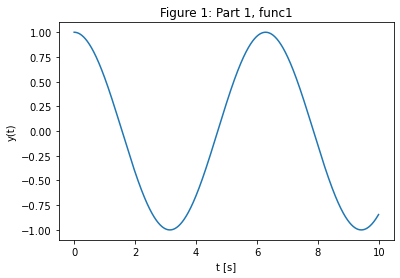
\includegraphics[width=0.55\textwidth]{Figure1.png}\\
The purpose producing Figure 1 was to develop a way of handing a function applied piece-wise to a sequence of numbers, which were the evenly spaced intervals of t.  The steps used were 0.01, and if they were lower, then the graph would appear jagged.

\subsection*{Part 2}
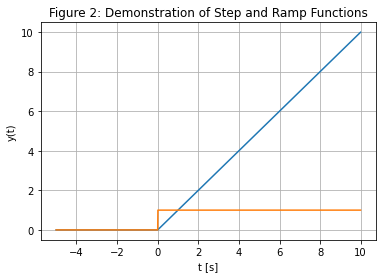
\includegraphics[width=0.55\textwidth]{Figure2.png}\\
In Figure 2, the orange line is the result of applying the unit step function, while the blue line is applying the ramp function.\\
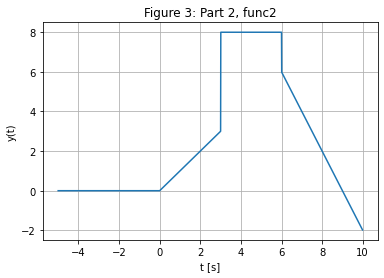
\includegraphics[width=0.55\textwidth]{Figure3.png}\\
In Figure 3, there are many ramps and step functions added together with scaling and time shifting. This can be represented by the equation:
\[func2(t) = r(t)-r(t-3)+5u(t-3)-2u(t-6)-2r(t-6)\]
In the Python code, the equation was stored as a function, so that variations could be easily created. and the output was
\[y=func2(t)\]\\

\subsection*{Part 3}
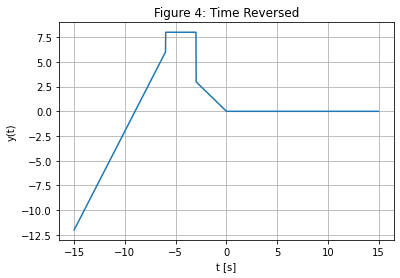
\includegraphics[width=0.55\textwidth]{Figure4.png}\\
Figure 4 is time reversed about the origin, and it was computed in python with the line \[y = func2(-t)\]\\

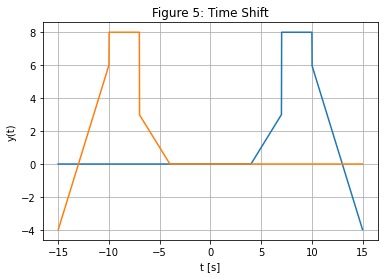
\includegraphics[width=0.55\textwidth]{Figure5.png}\\
Figure 5 shows time-shift as well as time reversal. The blue is \[y = func2(t-4)\] and the orange is \[y = func2(-t-4)\]\\

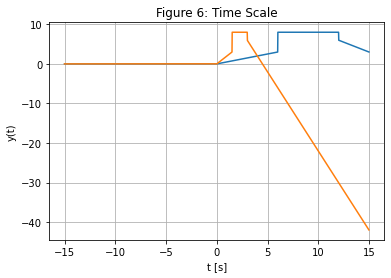
\includegraphics[width=0.55\textwidth]{Figure6.png}\\
Figure 6 shows time scaling. The blue is \[y = func2(t/2)\] and the orange is \[y = func2(t*2)\]\\

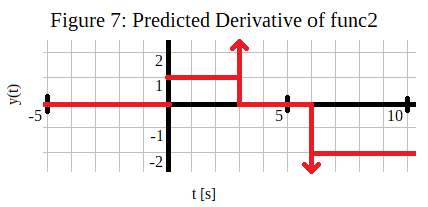
\includegraphics[width=0.55\textwidth]{Figure7.png}\\
Figure 7 is the predicted graph based on the mathematical equation for func2.\\

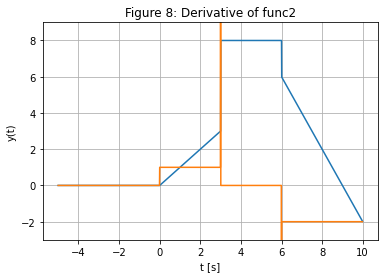
\includegraphics[width=0.55\textwidth]{Figure8.png}~\\
Figure 8 the derivative of func2. The blue is \[y = func2(t)\] and the orange is discrete derivative \[y =  \frac{d}{dt}( {func2(t*2)})\]
With the discrete derivative in the library numpy, the y.diff() will reduce the array size by one, which made the plotting fail with the library matplotlib due to miss-matched array lengths.  additionally, when working with discrete differential, you have to keep in mind the time interval and divide by diff(func(t)) by diff(t)

\section{Error Analysis}\label{sec:res}
Because of the use of discrete values, there is inherently a disconnect with the mathematical functions.  however when the step size is small enough, then you eventually reach a good enough when trying to distinguish the equation from the array of points.

\section{Questions}\label{sec:res}

\Q 1. Are the plots from Part 3 Task 4 and Part 3 Task 5 identical? Is it possible for them to match? Explain why or why not.
\A The hand drawn plot is a representation of mathematics while the python plot is a representation of data points. They appear close but are not identical

\Q 2. How does the correlation between the two plots (Part 3 Task 4 and Part 3 Task 5 ) change if you were to change the step size within the time variable in task 5? Explain why this happens.
\A2 When the interval between data points increases, the more jagged and less information is presented, this will cause erratic changes the noise that would be information cannot be parsed from the large time gaps.  This will make the two graphs to become less nearly-identical to clearly different as the interval increases.
\\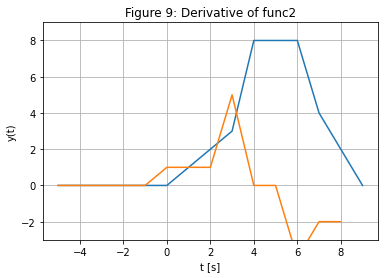
\includegraphics[width=0.55\textwidth]{Figure9.png}\\
In figure 9, the details that are the spikes are smoothed out and cannot be properly determined, additionally the blue (original function) is constant at zero at the interval -1 to 1, but its orange line (discrete derivative of the original function) is non-zero.

\Q 3.Leave any feedback on the clarity of lab tasks, expectations, and deliverable
\A The format of the lab instructions was at first confusing  because there was a bit of duplication ("2.Deliverables Overview", "Deliverables" in each section, and in the tasks themselves.


\section{Conclusion}\label{sec:res}
When creating a model it can be useful to use discrete values for ease of storing and manipulating on a computer.  However you must keep in mind that your time steps are sufficient to detect important details.  On vary large data-sets, it may become unwieldy without optimizing time (i.e. dynamically changing time steps), but for smaller data-sets of simple circuits it is trivial. performing computations on the large arrays of discrete values is way faster than by doing it by hand or creating a line of best fit to make a mathematical model.
Functions that do not originally exist, or functions with many steps can be automated as well, such as the case where the complicated func2 was composed of many transformed/translated step and ramp functions.


%\lipsum[7-8]\cite{knuthwebsite}
%===========================================================
%===========================================================
\bibliographystyle{ieeetr}
\bibliography{refs}
\end{document} 
Annotations











